\chapter{Project Structure \& Implementation}
\label{ch:implementation}

\section{Software Architecture}

The codebase is organized by pipeline stage into a small number of top-level directories, rather than around a class hierarchy. Figure~\ref{fig:pipeline_flow} shows the full flow from raw data to a frozen, evaluated model.

\begin{figure}[htbp]
\centering
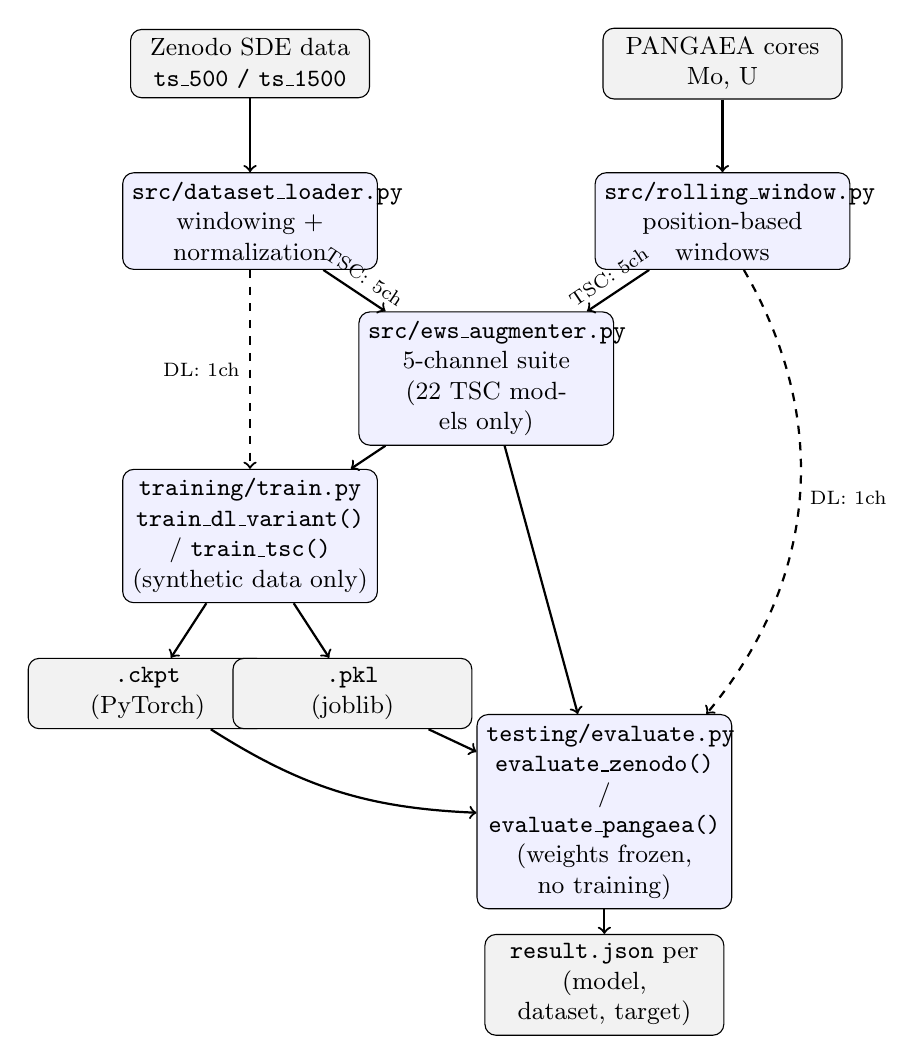
\begin{tikzpicture}[
    box/.style={draw, rounded corners, align=center, minimum height=0.9cm, text width=3.0cm, fill=blue!6, font=\small},
    io/.style={draw, rounded corners, align=center, minimum height=0.8cm, text width=2.8cm, fill=gray!10, font=\small},
    lbl/.style={font=\scriptsize, midway},
]
\node[io] (zenodo) at (0,10) {Zenodo SDE data\\ \texttt{ts\_500 / ts\_1500}};
\node[io] (pangaea) at (6,10) {PANGAEA cores\\ Mo, U};

\node[box] (prep) at (0,8) {\texttt{src/dataset\_loader.py}\\ windowing + normalization};
\node[box] (rolling) at (6,8) {\texttt{src/rolling\_window.py}\\ position-based windows};

\node[box] (feat) at (3,6) {\texttt{src/ews\_augmenter.py}\\ 5-channel suite\\ (22 TSC models only)};

\node[box] (train) at (0,4) {\texttt{training/train.py}\\ \texttt{train\_dl\_variant()} / \texttt{train\_tsc()}\\ (synthetic data only)};

\node[io] (ckptdl) at (-1.3,2) {\texttt{.ckpt}\\ (PyTorch)};
\node[io] (ckpttsc) at (1.3,2) {\texttt{.pkl}\\ (joblib)};

\node[box] (eval) at (4.5,0.5) {\texttt{testing/evaluate.py}\\ \texttt{evaluate\_zenodo()} / \texttt{evaluate\_pangaea()}\\ (weights frozen, no training)};

\node[io] (results) at (4.5,-1.7) {\texttt{result.json} per\\ (model, dataset, target)};

\draw[->, thick] (zenodo) -- (prep);
\draw[->, thick] (pangaea) -- (rolling);

% DL path: raw single channel, bypasses feat entirely
\draw[->, thick, dashed] (prep) -- node[lbl, left]{DL: 1ch} (train);
\draw[->, thick, dashed] (rolling) to[bend left=35] node[lbl, right]{DL: 1ch} (eval);

% TSC path: through feat, 5 channels
\draw[->, thick] (prep) -- node[lbl, above, sloped]{TSC: 5ch} (feat);
\draw[->, thick] (rolling) -- node[lbl, above, sloped]{TSC: 5ch} (feat);
\draw[->, thick] (feat) -- (train);
\draw[->, thick] (feat) -- (eval);

\draw[->, thick] (train) -- (ckptdl);
\draw[->, thick] (train) -- (ckpttsc);
\draw[->, thick] (ckptdl) to[bend right=15] (eval);
\draw[->, thick] (ckpttsc) -- (eval);
\draw[->, thick] (eval) -- (results);
\end{tikzpicture}
\caption{The actual pipeline flow, by file and function. Deep-learning models (dashed edges) read the raw, single-channel window directly; the 22 classical TSC models (solid edges through \texttt{ews\_augmenter.py}) see the 5-channel expansion instead -- the same fork described in Chapter~\ref{ch:methodology}, Section~\ref{sec:dl_architectures}. \texttt{training/train.py} only ever consumes the synthetic (Zenodo) side of this fork; \texttt{testing/evaluate.py} is the only place PANGAEA data is used, for both model families, and it never updates model weights.}
\label{fig:pipeline_flow}
\end{figure}

\subsection{Function-Based, Not Class-Hierarchy-Based}

The pipeline is organized as a small number of modules, each with a specific job, connected by plain function calls rather than an inheritance hierarchy of custom classes:

\begin{itemize}
    \item \textbf{Data loading} (\texttt{src/dataset\_loader.py}): one \texttt{EWSDataset} class (a direct subclass of \texttt{torch.utils.data.Dataset}, PyTorch's own base class -- not a custom base class of this project's own design) plus the free function \texttt{get\_dataloader()}; \texttt{load\_config()} itself is defined in \texttt{src/constants.py} and imported here. \texttt{src/pangea\_cleaner.py} handles the empirical cores as a set of free functions (\texttt{process\_core()} and others), not a loader class.
    \item \textbf{Feature engineering} (\texttt{src/ews\_augmenter.py}): a single function, \texttt{augment\_ews\_channels()}, that takes a batch of normalized windows and returns the 5-channel version. \texttt{src/data\_common.py} holds the smaller shared building blocks it and the data loaders both use: \texttt{normalize\_mean\_abs()}, \texttt{random\_left\_censor()}, \texttt{left\_pad\_to()}.
    \item \textbf{Model definitions} (\texttt{models/}): one file per deep-learning architecture (\texttt{cnn\_lstm.py}, \texttt{resnet.py}, \texttt{tcn.py}, and so on), each a direct \texttt{torch.nn.Module} subclass, plus \texttt{models/tsc.py}, which holds a dictionary of per-model settings (\texttt{TSC\_SPECS}) and a function that builds the requested classical-TSC model, either from whichever library backs it or, for the three models with no library implementation, from this thesis's own from-scratch code (Section~\ref{sec:tsc_libraries}).
    \item \textbf{Training} (\texttt{training/train.py}): two top-level functions, \texttt{train\_dl\_variant()} and \texttt{train\_tsc()}, selected by a command-line argument -- there is no single overarching \texttt{Trainer} class managing both paths.
    \item \textbf{Evaluation} (\texttt{testing/evaluate.py}): two top-level functions, \texttt{evaluate\_zenodo()} and \texttt{evaluate\_pangaea()}. This is also where empirical inference on the real cores happens -- there is no separate \texttt{inference.py} script; it is the same file and the same \texttt{--target pangaea} flag as the synthetic evaluation.
\end{itemize}

This is a deliberately flat design: adding a new model means adding one new file to \texttt{models/} and one entry to a config dictionary, not subclassing a shared base class. The trade-off is that some logic (e.g. the CPU/GPU split described in Section~\ref{sec:hpc}) is decided by which top-level script or SLURM array a job runs under, rather than by a shared class dispatching on model type.

This choice was checked against \citet{bury2021}'s own accompanying repository \citep{burygithub} rather than made in isolation: their codebase is organized the same way, as a set of standalone, task-specific scripts (\texttt{training\_data/} for data generation, \texttt{dl\_train/DL\_training.py} and \texttt{DL\_test.py} for training and evaluation, \texttt{test\_empirical/anoxia/} for the real-data test case) communicating through files on disk, not a shared class hierarchy either. The earlier, unverified description of this thesis's own architecture (an OOP hierarchy of loader/feature-engineer/trainer classes, corrected earlier in this rewrite) was not only inaccurate to this codebase -- it also did not match the reference implementation this thesis is built on.

\section{High-Performance Computing and SLURM}
\label{sec:hpc}

Training and evaluating dozens of models at two sequence lengths on synthetic data alone runs into the hundreds of thousands of training examples per model; on a single machine this would take an impractically long time. This thesis's experiments ran on a university HPC cluster, using SLURM \citep{yoo2003slurm} to schedule jobs.

\subsection{SLURM Array Jobs}

Rather than one script per model, each family of jobs (train all deep-learning models, train all TSC models, evaluate on Zenodo, evaluate on PANGAEA) is a single SLURM array script. Inside the script, plain bash indexes into a list of model names using \texttt{\$SLURM\_ARRAY\_TASK\_ID}:
\begin{quote}
\texttt{MODEL=\$\{MODELS[\$((SLURM\_ARRAY\_TASK\_ID / 2))]\}} \\
\texttt{DATASET=\$\{DATASETS[\$((SLURM\_ARRAY\_TASK\_ID \% 2))]\}}
\end{quote}
so a single \texttt{sbatch} submission launches one job per (model, dataset) pair. This mapping happens in the shell script itself, not inside any Python class.

\subsection{Hardware Split}

Deep-learning training and TSC training request different resources, because they have genuinely different bottlenecks. Deep-learning jobs (LSTM, CNN-LSTM, InceptionTime, ResNet, TCN, RNN-FCN, PatchTST) request a GPU partition with 4 CPU cores per job, since the bottleneck is GPU-bound matrix multiplication during backpropagation. Classical TSC jobs (MiniRocket, WEASEL2, and the rest) request a CPU-only partition with 16 CPU cores per job and no GPU, since these models use no backpropagation and their feature extraction (much of it implemented in Cython or Numba inside the underlying libraries) parallelizes across CPU cores instead.

\section{The Deep Learning Models: PyTorch}

Every deep-learning architecture (Chapter~\ref{ch:methodology}, Section~\ref{sec:dl_architectures}) is implemented in PyTorch \citep{paszke2019pytorch} as a direct \texttt{torch.nn.Module} subclass.

\subsection{Input Shape}

PyTorch's convolutional and recurrent layers expect a 3-dimensional tensor of shape \texttt{(batch\_size, channels, sequence\_length)}. A raw series of length $L$ starts as a flat 1D array; every deep-learning model in the roster is built to accept it directly, reshaped to \texttt{(batch\_size, 1, L)}, without the 5-channel feature suite -- that expansion (Chapter~\ref{ch:methodology}, Section~\ref{sec:dl_architectures}) applies only to the 22 classical TSC models, which see shape \texttt{(N, 5, L)} instead (Section~\ref{sec:tsc_libraries}).

\subsection{Dataset and DataLoader}

The synthetic training corpus is too large to hold entirely in memory at once. \texttt{EWSDataset} (\texttt{src/dataset\_loader.py}) implements PyTorch's standard lazy-loading pattern: \texttt{\_\_len\_\_()} reports how many examples exist, and \texttt{\_\_getitem\_\_(index)} loads and preprocesses exactly one example only when it is actually requested during training, rather than loading the whole dataset up front. Wrapping this in a standard \texttt{torch.utils.data.DataLoader} with multiple worker processes lets the next batch be prepared on the CPU while the GPU is still working on the current one.

\section{The Classical TSC Models}
\label{sec:tsc_libraries}

Of the 22 classical TSC models, 19 are instantiated from an existing open-source library rather than reimplemented; \texttt{models/tsc.py} builds each one from whichever library implements it, based on a per-model configuration dictionary (\texttt{TSC\_SPECS}). Three libraries back these 19, checked directly against the actual import statements in this repository:

\begin{itemize}
    \item \textbf{aeon} \citep{aeon2024}, a scikit-learn-compatible time series machine learning toolkit, backs the majority of the roster -- MiniRocket, MultiRocket, Rocket, Arsenal, RDST, WEASEL2, TDE, DrCIF, catch22, Proximity Forest, TSF, Shapelet Transform, Learning Shapelets, BOSS, CIF, and MrSQM among them.
    \item \textbf{pyts} \citep{pyts2020} backs the two models that are not in \texttt{aeon}'s catalogue used here: Bag-of-Patterns and SAX-VSM (\texttt{models/bakeoff\_dictionary.py}).
    \item \textbf{wildboar} backs gRSF (generalized Random Shapelet Forest), added to the roster this session and not covered by either of the other two libraries.
\end{itemize}

sktime, an earlier, related TSC library, is not used anywhere in this codebase -- an easy library to confuse with \texttt{aeon} (a number of \texttt{aeon} maintainers previously worked on sktime), so worth stating precisely rather than leaving ambiguous.

The remaining three models -- Time Series Bag of Features (TSBF), Learned Pattern Similarity (LPS), and Fast Shapelets -- have no maintained library implementation in Python, so they are built from scratch for this thesis (\texttt{models/bakeoff\_tsbf.py}, \texttt{models/bakeoff\_lps.py}, \texttt{models/bakeoff\_fastshapelet.py}), each using only \texttt{scikit-learn}'s \texttt{RandomForestClassifier} \citep{pedregosa2011sklearn} as a building block rather than a TSC-specific library. Each is a documented simplification of its original paper's algorithm (e.g. TSBF's fixed multi-scale interval segmentation is replaced with randomly positioned/length intervals in the style of \texttt{aeon}'s own TSF, already used elsewhere in this roster), and each file's own documentation states it was validated only against the UCR GunPoint dataset before use, since no reference implementation exists to check the output against directly.

For the ROCKET-family models specifically: \texttt{aeon}'s own implementation, not code written for this thesis, pairs the random/deterministic kernel feature extraction with a ridge-regression classifier internally (\texttt{RidgeClassifierCV} from \texttt{scikit-learn}, \citealp{pedregosa2011sklearn}) -- this thesis instantiates \texttt{aeon}'s classifier class directly and does not implement or choose that classifier backend itself.

\section{Serialization}

Once training finishes, model weights are saved to disk and never updated again. Deep-learning models save PyTorch's \texttt{state\_dict} (the layer weights, not the full class definition, to avoid version-compatibility problems later) with \texttt{torch.save}, as \texttt{.ckpt} files. Classical TSC models are Python objects from \texttt{aeon}/\texttt{pyts}/\texttt{wildboar} with no PyTorch dependency at all, and are saved with \texttt{joblib} as \texttt{.pkl} files instead.

\section{Empirical Evaluation on PANGAEA}

\texttt{testing/evaluate.py --target pangaea} is the script that runs a frozen, trained model against the real sediment cores. No training happens in this script -- every model is loaded from its saved checkpoint, and for deep-learning models, \texttt{model.eval()} is called to disable training-only behaviour (dropout, batch-norm update statistics) before any prediction is made.

\subsection{Generating a Probability Trajectory}

Rather than one classification for an entire core, the script computes a rolling series of predictions: \texttt{src/rolling\_window.py} places a fixed number of evenly-spaced windows (40 by default, \texttt{inference.prediction\_steps} in \texttt{config.yaml}) between the start of the usable pre-transition segment and the transition itself, and the model is run once per window. This gives a probability trajectory approaching the transition, not a single verdict -- not literally one prediction "at every available temporal step," but at a fixed, evenly-spaced set of 40 points per segment.

Each window's 4-class probability output, and the derived binary transition probability ($p_{\text{transition}} = 1 - P(\text{null})$), is written to that segment's \texttt{result.json}, alongside the classical rolling variance and lag-1 autocorrelation computed over the same window for comparison. These per-segment results are what every aggregate table and figure in this thesis is ultimately built from.
